
\subsection{Capital Regulation Before the Global Financial Crisis}



\subsubsection{Basel I}
\begin{itemize}
\item First put forth in 1988, Basel I was fully implemented by the end of 1992.
\item It includes:
    \begin{itemize}
    \item Credit risk
    \item Capital requirements
    \end{itemize}

\end{itemize}



\subsubsection{Credit risk-standardized approach}
\begin{itemize}
\item Risk-based capital ratio introduced risk-weighted assets(RWA). It included three categories:
    \begin{itemize}
    \item Those arising from on-balance sheet assets (excluding derivatives)
    \item Those arising for off-balance sheet items (excluding derivatives)
    \item Those arising from derivatives
    \end{itemize}
\item RWA: risk weights for on-balance-sheet items
    \begin{equation}
    \sum_{i=1}^{N} w_i L_i
    \end{equation}
\item $w_i$ is the risk weight, and $L_i$ is the principal amount.
\begin{table}[h]
    \centering
    \caption{Risk Weights and Asset Categories}
    \renewcommand{\arraystretch}{1.5} % 设置行距为1.5
    \begin{tabular}{|c|c|}
        \hline
        \textbf{Risk Weight (\%)} & \textbf{Asset Category} \\
        \hline
        0 & Cash, gold bullion, claims on OECD governments such as Treasury bonds or insured residential mortgages \\
        \hline
        20 & Claims on OECD banks and OECD public sector entities such as securities issued by U.S. government agencies or claims on municipalities \\
        \hline
        50 & Uninsured residential mortgage loans \\
        \hline
        100 & All other claims such as corporate bonds and less-developed country debt, claims on non-OECD banks \\
        \hline
    \end{tabular}
\end{table}

\item Example

Niu and Son's Bank holds \$100 million of Oman's debt (lessdeveloped country), \$100 million of corporate bonds, \$50 million of uninsured residential mortgage loans, \$50 million of gold bullion. Calculate the total of the risk weighted assets.

\item Answer


100 X 1.0 + 100 X 1.0 + 50 X 0.5 + 50 X 0= 225 million


\item RWA: risk weights for off-balance sheet items.

A credit equivalent amount （CEA） is calculated by applying a
conversion factor to the principal amount of the instrument.
For example, bankers' acceptances and guarantees are offbalance
sheet items.

    \begin{itemize}
    \item Bankers' acceptances have a conversion factor of 100%.
    \end{itemize}

\item RWA: derivatives under current exposure method

\item The credit equivalent amount is max (V, 0) + D (add-on amount).
    \begin{itemize}
    \item V is the current market value of the derivative, D is determined by a(add-on factor) and L(the principal amount). D accounts for changes of future market value.
    \end{itemize}
    \begin{table}[h]
        \centering
        \caption{Risk Weights by Remaining Maturity}
        \renewcommand{\arraystretch}{1.5} % 设置行距为1.5
        \begin{tabular}{|c|c|c|c|c|c|}
            \hline
            \textbf{Remaining Maturity (yr)} & \textbf{Interest rate} & \textbf{Exchange rate and gold} & \textbf{Equity} & \textbf{Precious metals except gold} & \textbf{Other commodities} \\
            \hline
            <1 & 0.0\% & 1.0\% & 6.0\% & 7.0\% & 10.0\% \\
            \hline
            1 to 5 & 0.5\% & 5.0\% & 8.0\% & 7.0\% & 12.0\% \\
            \hline
            >5 & 1.5\% & 7.5\% & 10.0\% & 8.0\% & 15.0\% \\
            \hline
        \end{tabular}
    \end{table}

\item Example

Niu and Son's Bank has entered into a \$100 million orange
juice forward contract with remaining life of 1.5 years.
Current value is 8 million and add-on factor is 12\%. Calculate
the credit equivalent amount.

\item Answer

8 + 12\% X 100 = 20 million

\item RWA: derivatives under original exposure method (only for interest rate and foreign exchange contracts)
\item The credit equivalent amount is D (add-on amount).
    \begin{itemize}
    \item D is determined by a(add-on factor either in original maturity or remaining maturity) and L(the principal amount).
    \end{itemize}
\item Total risk-weighted assets: calculated as following:
    \begin{equation}
    \sum_{i=1}^{N} w_i L_i + \sum_{j=1}^{M} w_j^* C_j
    \end{equation}
    \begin{itemize}
    \item $L_i$ is the principal of the $i_{th}$ on-balance-sheet asset and $w_i$
    is the risk weight for the asset.
    \item  $C_j$ is the credit equivalent amount for the $j_{th}$ derivative or
    other off-balance sheet item and $w_j$*is the risk weight of
    the counterparty for this $j_{th}$ item.
    \end{itemize}
\end{itemize}





\subsubsection{Capital requirement}
\begin{itemize}
\item Basel I required capital at least 8\% of the total RWA. It includes:
    \begin{itemize}
    \item Tier 1 Capital (core capital for solvency) at least 4\% of RWA
        \begin{itemize}
        \item Common Equity and disclosed reserves minus goodwill
        \item Noncumulative perpetual preferred stock
        \end{itemize}
    \item Tier 2 Capital ( recapitalization of entity in resolution/reduce the impact of failures on depositors)
        \begin{itemize}
        \item Loan loss reserves not allocated to impairment of certain assets
        \item Undisclosed reserves
        \item Hybrid instruments
        \end{itemize}
    \end{itemize}
\end{itemize}



\subsubsection{The 1995 and 1996 Amendments}
\begin{itemize}
\item Continuous efforts on unsolved issues pushed the updates of 1995 and 1996 amendments.

It includes:
    \begin{itemize}
    \item Credit risk-adjustment for derivatives
    \item Market risk
    \item Capital requirements
    \item Others
    \end{itemize}
    

\end{itemize}



\subsubsection{Credit risk-adjustment for derivatives}
\begin{itemize}
\item Netting: participants in the over-the-counter derivatives market began to sign an International Swaps and Derivatives Association(ISDA) master agreement.
\item Netting is a clause in ISDA master agreement, stating in the event of a default, all transactions are considered as a single transaction.
    \begin{itemize}
    \item If a company defaults on one transaction, it must default on all transactions.
    \end{itemize}

\item Contrast a financial institution has a portfolio of N derivatives with a particular counterparty and that the current value of the $i_{th}$ derivative $V_i$ .
    \begin{itemize}
    \item Without netting, the financial institution's exposure in the event of a default today is \(\sum_{i=1}^{N} \max(V_i, 0)\)
    \item With netting, it is \( \max\left(\sum_{i=1}^{N} V_i, 0\right) \)
    
    Without netting, the exposure is payoff from a portfolio of options.

    With netting, the exposure is payoff from an option on  portfolio.
    \end{itemize}
\item Net replacement ratio (NRR), is the ratio of the current exposure with netting to the current exposure without netting.
    \begin{equation}
    NRR = \frac{\max\left(\sum_{i=1}^{N} V_i, 0\right)}{\sum_{i=1}^{N} \max(V_i, 0)}
    \end{equation}
\item The credit equivalent amount (CEA) was modified to
    \begin{equation}
    \max\left(\sum_{i=1}^{N} V_i, 0\right) + (0.4 + 0.6 \times NRR) \sum_{i=1}^{N} D_i
    \end{equation}

\item Example
    \begin{itemize}
    \item Consider following portfolio of three derivatives that a bank has with a particular counterparty with the previous table on add-on amount.
    \end{itemize}
    \begin{table}[h]
        \centering
        \caption{Transaction Details}
        \renewcommand{\arraystretch}{1.5} % 设置行距为1.5
        \begin{tabular}{|c|c|c|c|}
            \hline
            \textbf{Transaction} & \textbf{Principal, \(L\)} & \textbf{Current value, \(V\)} & \textbf{Add-on amount, \(a \cdot L_i\)} \\
            \hline
            3-year interest rate swap & 1000 & -60 & 5 \\
            \hline
            6-year foreign exchange forward & 1000 & 70 & 75 \\
            \hline
            9-month option on a stock & 500 & 55 & 30 \\
            \hline
        \end{tabular}
    \end{table}

\item Answer
    \begin{itemize}
    \item The current exposure with netting is -60 + 70 + 55 = 65. The current exposure without netting is 0 + 70 + 55 = 125. Net replacement ratio is 65/125 =0.52. The total of the add-on amounts, \(\sum_{i=1}^{N} a_i L_i \text{ is } 5 + 75 + 30 = 110.\).
    \item The credit equivalent amount when netting is 65 + (0.4 + 0.6 x 0.52) x 110 = 143.32. Without netting, the credit equivalent amount is 125 + 110 = 235.
    \item If the risk weight is 0.2, the risk-weighted assets with netting is 0.2 X 143.32 = 28.66. Without netting, it is 0.2 x 235 = 47.
    \end{itemize}
\end{itemize}



\subsubsection{Market risk}
\begin{itemize}
\item Market risk capital charge for trading book


\begin{table}[h]
    \centering
    \caption{Comparison of Trading Book and Banking Book}
    \renewcommand{\arraystretch}{1.5} % 设置行距为1.5
    \begin{tabular}{|c|c|c|}
        \hline
        \textbf{ } & \textbf{Trading book} & \textbf{Banking book} \\
        \hline
        Purpose & Held for trading & Held to maturity \\
        \hline
        Time horizon & Short & Long \\
        \hline
        Risk type & Market risk & Credit risk \\
        \hline
        Confidence level & 99\% VaR & 99.9\% VaR \\
        \hline
        Example & marketable securities, most derivatives held by the bank for trading & Bank loans, some debt securities \\
        \hline
    \end{tabular}
\end{table}


\item It details the separate treatment of general market risk and specific risk
    \begin{itemize}
    \item MR (general market risk): general movements in market prices(such as interest rate risk).
    \item SR (specific risk): driven by idiosyncratic changes in a specific position's value(such as changes in a firm's credit spread or a firm's stock price).
    \end{itemize}
\item Corporate bonds are exposed to interest rate risk, captured by MR, and credit risk, captured by the SR.
\item Two approaches to calculate market risk capital
    \begin{itemize}
    \item Standardized approach
    \item Internal model-based approach
    \end{itemize}
\end{itemize}


\subsubsection{Market risk-standardized approach}
\begin{itemize}
\item The approach assigns capital separately to each item. It ignores correlations between items and assumes perfectly correlated.
    \begin{itemize}
    \item It details separately for five categories of positions
        \begin{itemize}
        \item Fixed income securities and interest rate derivatives except options;
        \item Equity securities and equity derivatives other than options;
        \item Foreign exchange;
        \item Commodities;
        \item All types of options
        \end{itemize}
    \end{itemize}
\end{itemize}


\subsubsection{Market risk-internal model-based approach}
\begin{itemize}
\item Internal model-based approach embodied a major change in philosophy by permitting banks to use internally developed risk measures as the inputs to formulas specified by regulators.
\item Total capital for trading assets= 0.08*12.S* total (MR+ SR)

    \begin{equation}
    MR = \max\left(VaR_{t-1}, m_c \times VaR_{avg}\right)
    \end{equation}
    \begin{itemize}
    \item VaR calculated with 10-day time horizon/99\% confidence level.
        \begin{itemize}
        \item It means a 1\% chance of being exceeded over a 10-day period, $m_c$ is a multiplicative factor with the minimal value of 3.
        \end{itemize}
    \end{itemize}
\end{itemize}


\subsubsection{Market risk-specific risk}
\begin{itemize}
\item Total capital for trading assets= 0.08*12.S* total (MR+ SR)
    \begin{itemize}
    \item Capital for specific risk, which was required for fixed income, equity instruments, and derivatives, could be determined using either the standardized approach or the bank's internal models.
        \begin{itemize}
        \item In using internal models, banks calculate a 10-day 99\% VaR for SR. T he multiplier was 4 rather than 3 and capital for specific risk could not be less than half of capital calculated using the standardized approach.
        \end{itemize}
    \end{itemize}
\end{itemize}


\subsubsection{Capital requirements}
\begin{itemize}
\item Tier 3 capital
    \begin{itemize}
    \item Composed mainly of unsecured subordinated debt with an original maturity of at least 2 years, that could be used to meet part of market risk capital requirement.
    \end{itemize}
\end{itemize}


\subsubsection{Others}
\begin{itemize}
\item Back-testing
    \begin{itemize}
    \item Banks are required to daily back-testing one-day, 99\%VaR over the previous 250 days.
    \item Number of exception in this back-testing determines mc.
        \begin{itemize}
        \item Less than 5 （0-4 days）, me equals 3.
        \item 5, 6, 7, 8, or 9, me equals 3.4, 3.5, 3.65, 3. 75, and 3.85, respectively.
        \item More than 9 （10 or more days）, me equals 4.
        \end{itemize}
    \end{itemize}
\end{itemize}




\subsubsection{BASEL II}
\begin{itemize}
\item In 1999, the Basel Committee proposed new rules which was known as Basel II. The final revision was in 2004. It includes:
    \begin{itemize}
    \item Three pillars
    \item Credit risk
    \item Operation risk
    \end{itemize}
\end{itemize}


\subsubsection{Three pillars by BCBS}
\begin{itemize}
\item Basel II developed three pillars: minimum capital requirements, supervisory review process, and market discipline.
    \begin{itemize}
    \item Regulatory capital for Pillar 1 determines the minimum level of capital that banks need to cover the risk of unexpected losses from credit, market, and operational risks, and the minimum ratios required.
    \item Supervisory review process: Pillar 2 includes additional capital requirements ("add-ons") to Pillar 1 capital for the specific risk profile of a regulated entity.
    \item Market discipline: Disclose qualitative and quantitative information.
    \end{itemize}
\end{itemize}


\subsubsection{Credit risk}
\begin{itemize}
\item For credit risk, Basel II specified three approaches:
    \begin{itemize}
    \item Standardized approach
    \item Foundation internal ratings based （IRB） approach
    \item Advanced IRB approach
    \end{itemize}
\end{itemize}


\subsubsection{Credit risk-standardized approach}
\begin{itemize}
\item It is used by banks that are not sufficiently sophisticated.
\item Standardized approach is similar to Basel I except for the calculation of risk weights.
    \begin{itemize}
    \item Under Basel I, the headline risk weights depended on asset type and nationality of the obligor;
    \item Under Basel II, the headline risk weights depended on obligor type and rating for some obligor types, and on asset type for others.
    \end{itemize}
\item Risk weights as a percent of principal

\begin{table}[h]
    \centering
    \caption{Risk Weights by Credit Rating}
    \renewcommand{\arraystretch}{1.5} % 设置行距为1.5
    \begin{tabular}{|c|c|c|c|c|c|c|}
        \hline
        \textbf{ } & \textbf{AAA to AA -} & \textbf{A+ to A -} & \textbf{BBB+ to BBB -} & \textbf{BB+ to B -} & \textbf{Below B -} & \textbf{Unrated} \\
        \hline
        Country & 0 & 20 & 50 & 100 & 150 & 100 \\
        \hline
        Banks & 20 & 50 & 50 & 100 & 150 & 50 \\
        \hline
        Corporations & 20 & 50 & 100 & 100 & 150 & 100 \\
        \hline
    \end{tabular}
\end{table}

\item Example
    \begin{itemize}
    \item Assets of Niu and Son's Bank includes \$100 million of bank's bond rated AA, \$200 million of government bond rated A+, and \$300 million of corporate bond rated BB-. Calculate riskweighted assets under Basel II standardized approach.
    \end{itemize}
    
\item Answer
    \begin{itemize}
    \item 100 X 20\% + 200 X 20\% + 300 X 100\% = 360 million
    \end{itemize}
    
\end{itemize}


\subsubsection{Credit risk-mitigants}
\begin{itemize}
\item Collateral: two approaches can adjust risk weights.
    \begin{itemize}
    \item The first is termed the simple approach and is similar to an approach used in Basel I.
        \begin{itemize}
        \item For the part of the exposure covered by the collateral, the risk weight of the collateral is used.
        \item For any exposure not covered by the collateral, the risk weight of the counterparty is used.
        \item The minimum risk weight is 20\% except for sovereign debt.
        \end{itemize}
    \end{itemize}
\item Example
    \begin{itemize}
    \item Red Star bank has \$100 million exposure to Giant company. The exposure is secured by \$90 million of T-bond rated AAA with a risk weight of 0\%, and Giant company has a rating of A with a risk weight of 50\%. Calculate risk-weighted assets applicable to the exposure using the simple approach.
    \end{itemize}
\item Answer
    \begin{itemize}
    \item 90 X 0+ 10 X S0\% = 5 million
    \end{itemize}

\item The second is termed the comprehensive approach.
    \begin{itemize}
    \item Banks adjust the size of their exposure upward, and adjust the value of the collateral downward. The adjustments depend on the volatility of the exposure and the collateral.
    \item A new exposure equal to the excess of the adjusted exposure over the adjusted value of the collateral.
    \end{itemize}
\item Example
    \begin{itemize}
    \item Red Star bank has \$100 million exposure to Giant company. The exposure is secured by \$90 million of T-bond rated AAA with a risk weight of 0\%, and Giant company has a rating of A with a risk weight of 50\%. Exposure would increase 20\% and value of collateral would decrease 5\% in the future. Calculate risk-weighted assets under the comprehensive approach.
    \end{itemize}

\item Answer
    \begin{itemize}
    \item New exposure: 100 X 1.2 - 90 X 95\% = 34.5 million
    \item RWA: 34.SX50\% = 17.25 million
    \end{itemize}
\end{itemize}


\subsubsection{Credit risk-foundation internal ratings based approach}
\begin{itemize}
\item Capital requirement on VaR is calculated using a one-year time horizon and a 99.9\% confidence level.
    \begin{itemize}
    \item Expected loss is covered by financial products pricing.
    \item Unexpected loss would be solved by VaR.
        \begin{itemize}
        \item Capital required is VaR minus expected loss.
        \end{itemize}
    \end{itemize}
\end{itemize}


\subsubsection{Credit risk-foundation IRB approach}
\begin{itemize}
\item 
\textbf{Capital required:} 
\[
\sum_{i} (EAD_i \times LGD_i \times DR99.9_{i}) - EL
\]

    \begin{itemize}[label=\checkmark]
    \item EAD: The exposure at default (in dollars)
    \item LGD: The loss given default (expressed as a decimal)
    \item $DR99.9_{i}$ or WCDR: The default rate at the 99.9\textsuperscript{th} percentile for a large portfolio of assets of type \(i\).
    \item EL: \(\sum_{i}(EAD_i \times LGD_i \times PD)\)
    \end{itemize}
        \begin{figure}[H]
        \centering
        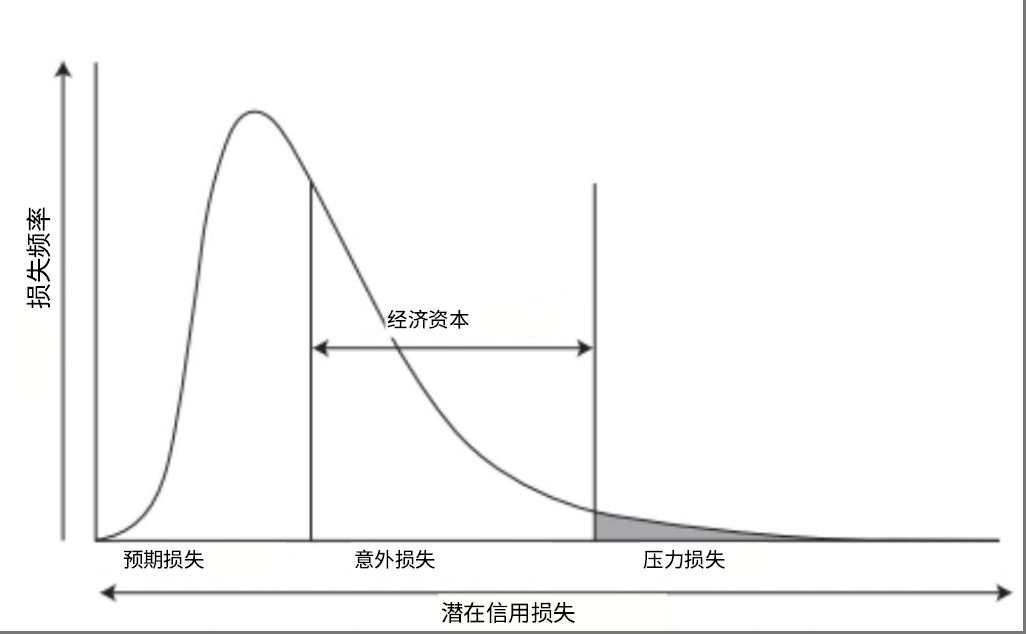
\includegraphics[width=0.8\textwidth]{images/潜在信用损失.png}
        \caption{潜在信用损失}
        \label{fig:label15}
        \end{figure}
\item Loss distribution, expected and unexpected loss, and capital
\item  The final version of capital calculation:  

RWA = 12.5 X EAD X LGD X （$DR99.9_i$ - PD）X MA

\begin{itemize}
    \item MA is the maturity adjustment, equals \(1 + \frac{(M - 2.5) \times b}{1 - 1.5 \times b}\).
    \item M is the maturity of the exposure.
    \begin{equation}
        DR99.9_{i} = N\left[N^{-1}(PD_i) - \sqrt{\rho} N^{-1}(0.001) \middle/ \sqrt{1 - \rho}\right]
        \end{equation}
    \end{itemize}
\item It is obvious that $DR99.9_i$ increases as the copula correlation between each pair of obligors increases and as the probability of default increases.
\item If the copula correlation is 0, $DR99.9_i$ is equal to PD.

\begin{table}[h]
    \centering
    \caption{Values of PD for Different Correlation Coefficients}
    \renewcommand{\arraystretch}{1.5} % 设置行距为1.5
    \begin{tabular}{|c|c|c|c|c|}
        \hline
        \textbf{$\rho$} & \textbf{PD=0.001} & \textbf{PD=0.005} & \textbf{PD=0.01} & \textbf{PD=0.02} \\
        \hline
        0 & 0.001 & 0.005 & 0.01 & 0.02 \\
        \hline
        0.2 & 0.028 & 0.092 & 0.146 & 0.226 \\
        \hline
        0.4 & 0.071 & 0.211 & 0.316 & 0.449 \\
        \hline
        0.6 & 0.135 & 0.387 & 0.542 & 0.705 \\
        \hline
    \end{tabular}
\end{table}

\item PD has inverse relationship with correlation ρ.
    \begin{equation}
    \rho = 0.24 - 0.12 \times \left( \frac{1 - e^{-50PD}}{1 - e^{-50}} \right)
    \end{equation}
    \begin{itemize}
    \item As a company becomes less creditworthy, its PD increases and its probability of default becomes more idiosyncratic and less affected by overall market conditions.
    \end{itemize}
\item Under the Foundation IRB approach, banks supply PD while LGD, EAD, and M are supervisory values set by the Basel Committee.
    \begin{itemize}
    \item The EAD is calculated similar to the credit equivalent amount (CEA) under Basel I. It includes the impact of netting.
    \item MA is set to 2.5 in most cases.
    \end{itemize}
\item Under the advanced IRB approach, banks supply their own estimates of the PD, LGD, EAD, and M for corporate, sovereign, and bank exposures.
\item For retail exposure, advanced IRB approach is used, but no maturity adjustment. Correlation are lower for retail than for wholesale exposure
\end{itemize}


\subsubsection{Operational risk}
\begin{itemize}
\item Three approaches to calculating capital for operational risk:
    \begin{itemize}
    \item Basic indicator approach (simplest)
    \item Standardized approach (middle)
    \item Advanced measurement approach (most sophisticated)
    \end{itemize}
\end{itemize}


\subsubsection{Operational risk-standardized approach}
\begin{itemize}
\item Basic indicator approach (BIA)

Capital calculation is a simple calculation of the average gross revenue for the past three years, multiplied by 15\%.

\item \( K_{BIA} = \frac{\sum_{i=1}^{n} G_{I_i} \times \alpha}{n} \)
    \begin{itemize}
    \item GI: annual positive gross income
    \item n: number of years in which gross income was positive
    \item $\alpha$ : 15\%
    \end{itemize}

\item Example

Niu and Son's Bank had annual gross revenue for the past three years as 200 million, -50 million, and 150 million respectively. Calculate the operational risk capital requirement.


\item Answer
    \begin{equation}
    K_{BIA} = \frac{(200 + 150) \times 15\%}{2} = 26.25
    \end{equation}

\item Standardized approach (SA)

It captures operational risk factors, because different types of business activities carry different levels of operational risk.
    \begin{itemize}
    \item Beta factor($\beta$) is a fixed percentage, which reflects the level of the gross income for each of the eight business lines.
    \end{itemize}
\item \begin{equation}
    K_{TSA} = \frac{\sum_{years \, 1-3} \max\left[\sum(GI_{1-8} \times \beta_{1-8}), 0\right]}{n}
    \end{equation}
    \begin{itemize}
        \item $GI_i$ : annual gross income in a given year
        \end{itemize}
\item beta factors
    \begin{itemize}
    \item 投行结算 （18\%）
    \item 商行托管 （15\%）
    \item 零经资产 （12\%）
    \end{itemize}
    \begin{table}[h]
        \centering
        \caption{Business Lines and Beta Factors}
        \begin{tabular}{|l|c|}
            \hline
            \textbf{Business Lines} & \textbf{Beta Factors} \\
            \hline
            Corporate finance (IB) & 18\% \\
            Trading and sales (IB) & 18\% \\
            Payment and settlement & 18\% \\
            Commercial banking & 15\% \\
            Agency (\& custody) service & 15\% \\
            Retail banking & 12\% \\
            Retail brokerage & 12\% \\
            Asset management & 12\% \\
            \hline
        \end{tabular}
    \end{table}

\item Example
    \begin{itemize}
    \item Niu and Son's Bank had three lines of business for the past 3 years to do business (in \$million).
    
    \begin{table}[h]
        \centering
        \caption{Business Line Performance Over Three Years}
        \begin{tabular}{|l|c|c|c|}
            \hline
            \textbf{Business Line} & \textbf{Year 1} & \textbf{Year 2} & \textbf{Year 3} \\
            \hline
            Retail banking & 10 & 10 & 20 \\
            Commercial banking & 10 & 10 & 20 \\
            Settlement and payment service & -20 & 0 & 10 \\
            \hline
        \end{tabular}
    \end{table}
    \item Calculate the operational risk capital requirement.
    \end{itemize}
    

\item Answer
    \begin{itemize}
    \item TSA capital charge per year:
    \begin{table}[h]
        \centering
        \caption{Business Line Calculations Over Three Years}
        \begin{tabular}{|l|c|c|c|}
            \hline
            \textbf{Business Line} & \textbf{Year 1} & \textbf{Year 2} & \textbf{Year 3} \\
            \hline
            Retail banking & \(10 \times 12\% = 1.2\) & \(10 \times 12\% = 1.2\) & \(20 \times 12\% = 2.4\) \\
            \hline
            Commercial banking & \(10 \times 15\% = 1.5\) & \(10 \times 15\% = 1.5\) & \(20 \times 15\% = 3.0\) \\
            \hline
            Settlement and payment service & \(-20 \times 18\% = -3.6\) & \(0 \times 18\% = 0\) & \(10 \times 18\% = 1.8\) \\
            \hline
            Total & \(-0.9\) & \(2.7\) & \(7.2\) \\
            \hline
        \end{tabular}
    \end{table}
    \item \begin{equation}
        K_{TSA} = \frac{2.7 + 7.2}{2} = 4.95 \text{ million}
        \end{equation}
    \end{itemize}

\item Advanced measurement approach (AMA) estimates
distribution of losses in seven categories that incorporates estimates of both the incidence of operational loss events and their severity.

\item Two broad approaches are most popular:
    \begin{itemize}
    \item 1. A parametric and Monte Carlo approach: data parameterize the probability distribution for incidence/severity to combine, producing large simulated loss observations to the value in 99.9th.
    \item 2. A scenario analysis approach: several detailed scenarios to measure operational losses in each scenario. Scenario analysis has the advantage of generating informative narratives and being forward-looking.
    \end{itemize}
\item Others
    \begin{itemize}
    \item The capital requirement under AMA is based on one-year time horizon, 99.9\% confidence level VaR.
    \item  Model must capture all expected and unexpected losses.
    \item Four elements should be included, internal loss data, external loss data, scenario analysis, and business environment \& control.
    \item Bank must defend correlation assumptions in its AMA model.
    \item Bank considers risk mitigating factors: may offset at most 20\% of the operational risk capital charge with insurance compensation or claim instead of insurance premium.
    \end{itemize}

\end{itemize}


\subsubsection{Solvency II}
\begin{itemize}
\item The long-standing regulatory framework for insurance companies in the European Union is known as Solvency I, is the process of being replaced by Solvency II.
\item In the United States and the European Union, Solvency II establishes capital requirements for operational, investment, and underwriting risks of insurance companies.
\item Solvency II is the "Basel II" for insurance company, and it has many similarities to Basel II.
    \begin{itemize}
    \item Three Pillars: Pillar 1 quantitative requirement. Pillar 2 internal governance and official supervision. Pillar 3 disclosure and transparency.
    \item Underwriting risk, credit and market risk, and operational risk are all considered. Underwriting risk is further detailed to risks arising from life insurance, P\&C (property \& casualty), health insurance.
    \end{itemize}

\end{itemize}



\subsubsection{Solvency II: SCR and MCR}
\begin{itemize}
\item If its capital falls below SCR (solvency capital requirement) level, a restore capital plan should be delivered to supervisor. Supervisors force the insurance company to take particular measures to correct the situation.
\item MCR (minimum capital requirement) is regarded as an absolute minimum level of capital. If capital drops below the MCR level, supervisors may prevent the insurance company from taking new business, or force the insurance company into resolution, transferring its policies to another company.
\end{itemize}



\subsubsection{Solvency II: SCR calculating}
\begin{itemize}
\item Calculating the SCR has two ways: standardized approach and internal models approach.
\item Internal models approach is calculated with VaR concept with one-year and 99.5\% confidence limit.
\item Capital structure:
    \begin{itemize}
    \item Tier 1 capital (equity, retained earnings and equivalents);
    \item Tier 2 capital (liabilities subordinated to policyholders);
    \item Tier 3 capital (subordinated to policyholders).
    \end{itemize}
    
\end{itemize}




\subsection{Solvency, Liquidityand Other Regulation After the Global Financial Crisis}


\subsubsection{Basel II.5}
\begin{itemize}
\item In the 2008 crisis, The Basel Committee recognized minimum capital under the market risk amendment were inadequate for the trading-book. It implemented updated rules by the end of 2011. 
\item It includes:
    \begin{itemize}
    \item Stressed VaR
    \item Incremental risk charge
    \item Comprehensive risk capital
    \end{itemize}
\end{itemize}



\subsubsection{Market risk-stressed VaR}
\begin{itemize}
\item Stressed VaR: Basel 11.5 requires banks to calculate two VaRs. One is the usual VaR (based on the previous one to four years of market movements). The other is stressed VaR .
\item Stressed VaR is determined by basing calculations on how market variables moved during the one year (250-day) period from the most recent seven years that was most stressful for its current portfolio, rather than on how they moved during the past one to four years.
\item The two VaR measures are combined to calculate capital charge.

    \begin{equation}
    \max\left(VaR_{t-1}, m_c \times VaR_{avg}\right) + \max\left(sVaR_{t-1}, m_s \times sVaR_{avg}\right)
    \end{equation}

    \begin{itemize}
        \item $VaR_{t-i}$ and $sVaR_{t-i}$ are usual VaR and stressed VaR with 10-day time horizon, 99\% confidence level on the previous day.
        \item $VaR_{avg}$ and $sVaR{avg}$ are the average of VaR and stressed VaR with 10-day time horizon, 99\% confidence level over the previous 60 days.
        \item $m_s$ and $m_c$ are multiplicative factors that are determined by bank supervisors and are between 3 to 4.
        \end{itemize}
\item Example

Niu and Son's Bank calculated that the usual VaR for the previous day and average one covering the last 60 days are 18 million and 5.2 million, and the stressed VaR for the previous day and average one covering the last 60 days are 26.4 million and 11.3 million. Based on the backtesting result, Niu and Son's discovered the me is 3 and ms is 3.5. Calculate the total market risk capital charge.

\item Answer

Max (18, 5.2 × 3) + max (26.4, 11.3 × 3.5) = 18 + 39.55 = 57.55

\end{itemize}



\subsubsection{Market risk-lRC}
\begin{itemize}
\item Incremental risk charge: the specific risk charge was intended to capture default and reaction to regulatory arbitrage opportunities between the banking and trading book.The Basel Committee named incremental default risk charge （IDRC）

    \begin{itemize}
    \item the internal model of default risk calibrated to the same 99.9th percentile at a one-year horizon.
    \end{itemize}

\item Later, the committee had realized that most losses with credit risk due to changes in ratings, credit spreads, or liquidity, not defaults.
    \begin{itemize}
    \item As a result, IDRC was widened to incremental risk charge (IRC).
    \end{itemize}
    
\item Comprehensive risk charge (CRC): An assumption in Basel II is that the correlation parameter is constant across obligors and over time. The assumption is wrong for instruments in the correlation book (securitizations/re-securitizations/ relating derivatives) .
\item Such correlation-sensitive instruments put assets in SPV and create tranches differ in seniority. Correlations changes have large effects on the tranches.
    \begin{itemize}
    \item The Basel Committee addressed the issue by replacing the IRC and specific risk charge with comprehensive risk (CR) charge for the correlation book. Comprehensive risk charge can use in either standardized approach or internal model approach.
    \end{itemize}
\item standardized approach

\begin{table}[h]
    \centering
    \caption{Standardized Capital Charge for Correlation-Dependent Instruments}
    \begin{tabular}{|l|c|c|c|c|c|}
        \hline
        \textbf{Types of Instrument} & \textbf{AAA to AA-} & \textbf{A+ to A-} & \textbf{BBB+ to BBB-} & \textbf{BB+ to BB-} & \textbf{Below BB- or Unrated} \\
        \hline
        Securitization & 1.6\% & 4\% & 8\% & 28\% & 100\% \\
        \hline
        Resecuritization & 3.2\% & 8\% & 18\% & 52\% & 100\% \\
        \hline
    \end{tabular}
\end{table}
\item Internal model approach: If a bank is allowed to use an internal model, it must routinely perform rigorous stress tests.

\end{itemize}



\subsubsection{Basel III}
\begin{itemize}
\item After the global financial crisis, The Basal Committee submitted the proposals to remedy the deficiencies. The proposals were published in 2010 and 2011. It includes:
    \begin{itemize}
    \item Capital requirements
    \item Liquidity risk
    \item Counterparty credit risk
    \end{itemize}
\end{itemize}



\subsubsection{Capital requirements}
\begin{itemize}
\item Under Basel III, a bank's total capital consists of:
    \begin{itemize}
    \item Tier 1 capital includes：
        \begin{itemize}
        \item Tier 1 equity capital
        \item Additional Tier 1 capital
        \end{itemize}
    \item Tier 1 capital excludes: Goodwill, other intangibles, deferred tax assets and any shortfall of reserves relative to IRB expected losses.
    \item Tier 1 equity capital includes: common equity/retained earnings /a limited amount of minority interest and unrealized gains and losses
    \item Additional Tier 1 capital: unsecured, unguaranteed, noncumulative perpetual preferred equity instruments subordinated to depositors and subordinated debt, and callable only after 5 years or more/debt with appropriate triggers that cause conversion to equity or write-downs/ approved minority interest not included in Core Tier 1
    \end{itemize}
\item Under Basel III, a bank's total capital consists of:
    \begin{itemize}
    \item Tier 2 capital: protecting depositors and creditors after failure.
    \item Subordinated debt: unsecured, unguaranteed debt instruments subordinated to depositors and subordinated debt, with 5 years or more original maturity, and callable only after 5 years or more.
    \item General loan loss reserves: reserves not allocated to absorb losses on specific positions. Reserves included in capital are capped at 1.25\% of standardized approach RWAs, or 0.6\% of IRB RWAs
    \end{itemize}

\item Basel Committee refers common equity as "going-concern capital." When the bank is a going concern (i.e., has positive equity capital), common equity absorbs losses.
\item Tier 2 capital is referred to as "gone concern capital." When the bank is no longer a going concern (i.e., has negative capital), losses have to be absorbed by Tier 2 capital.
\item Tier 2 capital ranks below depositors in a liquidation. While Tier 2 capital remains positive, depositors should in theory be repaid.
\item The minimum capital requirements are as follows:
    \begin{itemize}
    \item 1. Tier 1 equity capital must be at least 4.5\% of risk weighted assets at all times.
    \item 2. Total Tier 1 capital (Tier 1 equity capital plus additional Tier 1 capital) must be at least 6\% of risk-weighted assets at all times.
    \item 3. Total capital (total Tier 1 plus Tier 2) must be at least 8\% of risk-weighted assets at all times.
    \end{itemize}
\end{itemize}



\subsubsection{Capital requirements-buffers}
\begin{itemize}
\item Capital conservation buffer (CCB): Basel III requires capital conservation buffer in normal times consisting of further amount of core Tier 1 equity capital equal to 2.5\% of riskweighted assets
    \begin{itemize}
    \item It means the minimal value of Tier 1 equity capital ratio is 7\%, that of Tie 1 capital is 8.5\%, and that of total （Tier 1 plus Tier 2） is 10.5\%.
    \item The rationale is that large buffer is specified to further reduce the chance of failure.
    \end{itemize}

\item Countercyclical capital buffer (CCB): countercyclical capital buffer that varies at the discretion of national supervisors and is between O and 2.5\% of total risk-weighted assets and must be met with core Tier 1 equity capital. assets.
\item The rationales for CCB:
    \begin{itemize}
    \item Provide for macroprudential restraint of overheating, higher capital requirements tend to restrict credit supply by banks.
    \item The cost of capital: bank's cost of capital is smaller in good times than in bad times.
    \end{itemize}
\end{itemize}



\subsubsection{Capital requirements-G-SIBs buffer}
\begin{itemize}
\item The Financial Stability Board(FSB) became the body in which many changes in international standards were approved.
\item FSB publishes lists of G-SIB stands for global systemically important bank and G-S11 for insurer, whereas the SIFls means systemically important financial institutions.
\item National regulators designate banks that have not been classified as G-SIBs as domestic systematically important banks (D-SIBs).
\item The SI Fis are often presumed to be "too big to fail" and subjected to more regulation.
\item Standard of SI Fis depends on the effect that its failure could have on the global financial system.
\item G-SIBs are categorized according to whether the extra equity capital is 1\%, 1.5\%, 2\%, 2.5\%, or 3.5\% of risk-weighted assets.
\item Living wills: G-SIBs and D-SIBs are required to prepare detailed resolution plans when distressed, including how they would recapitalize and operate as a going concern.


\begin{figure}[H]
    \centering
    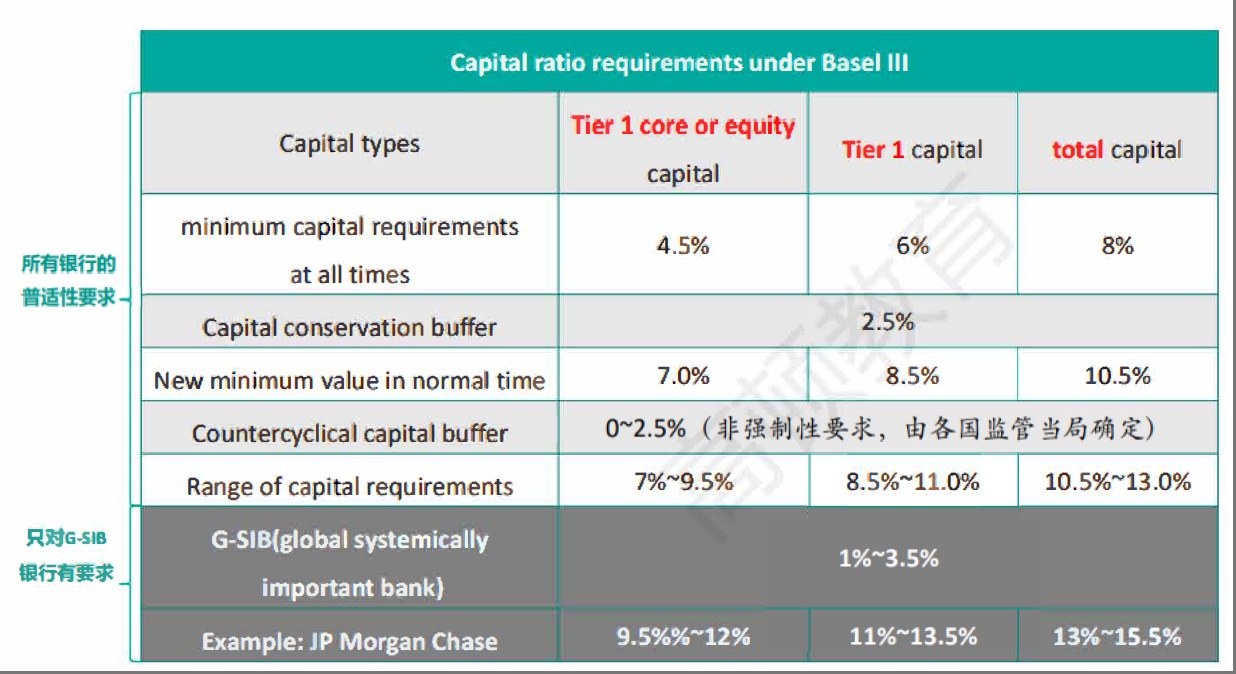
\includegraphics[width=0.8\textwidth]{images/CAPRAT.png}
    \caption{CAPRAT}
    \label{fig:label12}
    \end{figure}



\end{itemize}



\subsubsection{Capital requirements -leverage ratio}
\begin{itemize}
\item Basel III specifies a minimum leverage ratio of 3\% to supplement to the risk-based requirements.
\item he leverage ratio is the ratio of a Tier 1 capital to leverage exposure.
    \begin{itemize}
    \item Leverage exposure includes both on-balance-sheet assets and fractions of off-balance-sheet assets(e.g., derivatives or potential futures exposures).
    \end{itemize}
\end{itemize}



\subsubsection{Capital requirements- Cocos}
\begin{itemize}
\item Contingent convertible bonds: increase equity automatically when distress occurs, as triggers in the indenture are touched.
\item Common trigger is the ratio of Core Tier 1 Capital to RWA falls below a threshold, or regulator declares bank's nonviable.
\item Cocos may be included in Additional Tier 1 or Tier 2.
\item Economic benefits: As bonds, Cocos' cost is less than the cost of equity. Secondly, Cocos do not appear in the equity in normal time, a bank can report a higher ROE.
\end{itemize}



\subsubsection{Liquidity risk}
\begin{itemize}
\item Basel III has introduced requirements involving two liquidity ratios that are designed to ensure that banks can survive liquidity pressures.
\item Liquidity coverage ratio (LCR)
\item The bank has more liquid assets than it needs to meet a 30- day period of liquidity disruptions.
\item Net stable funding ratio (NSFR)
\item It focuses on liquidity management over a period of one year.
\end{itemize}



\subsubsection{Liquidity risk: LCR}
    \begin{equation}
    \text{Liquidity (LCR)} = \frac{\text{High-Quality Liquid Assets}}{\text{Net Cash Outflows in a 30-Day Period}}
    \end{equation}
\begin{itemize}
\item The 30-day period might include the following acute stress: a downgrade of the bank's debt by 3 notches (from AA to A), a partial loss of deposits, a complete loss of wholesale funding, increased haircuts on secured funding (collateral asset are not valued as highly), and drawdowns on lines of credit.
\item Basel III regulations require the ratio to be greater than 100\% so that the bank's liquid assets are sufficient to survive these pressures.
\end{itemize}



\subsubsection{Liquidity risk: : NSFR}
    \begin{equation}
    \text{Net Stable Funding Ratio (NSFR)} = \frac{\text{Amount of Stable Funding}}{\text{Required Amount of Stable Funding}}
    \end{equation}
\begin{itemize}
\item The numerator is calculated by multiplying each category of funding (liability and equity) by an available stable funding (ASF) factor, reflecting their stability.
\item The denominator is calculated from the items requiring funding (asset). Each category of these is multiplied by a required stable funding (RSF) factor to reflect the permanence of the funding required.
\item Basel III regulations require the ratio to be greater than 100\%.

\begin{table}[H]
    \centering
    \caption{ASF Factor}
    \renewcommand{\arraystretch}{1.5} % 设置行距为1.5
    \begin{tabular}{|c|p{14cm}|}
        \hline
        \textbf{ASF Factor} & \textbf{Category} \\
        \hline
        100\% & Tier 1 and Tier 2 capital, preferred stock and borrowing with a remaining maturity greater than one year \\
        \hline
        90\% & ``Stable'' demand deposits and term deposits with remaining maturity less than one year provided by retail or small business customers \\
        \hline
        80\% & ``Less Stable'' demand deposits and term deposits with remaining maturity less than one year provided by retail or small business customers \\
        \hline
        50\% & Wholesale demand deposits and term deposits with remaining maturity less than one year provided by nonfinancial corporates, sovereigns, central banks, multilateral development banks, and public sector entities \\
        \hline
        0 & All other liability and equity categories \\
        \hline
    \end{tabular}
\end{table}

\begin{table}[H]
    \centering
    \caption{RSF Factor}
    \renewcommand{\arraystretch}{1.5} % 设置行距为1.5
    \begin{tabular}{|c|p{14cm}|}
        \hline
        \textbf{RSF Factor} & \textbf{Category} \\
        \hline
        0\% & Cash, short-term instruments, securities, loans to financial entities if they have a residual maturity of less than one year \\
        \hline
        5\% & Marketable securities with a residual maturity greater than one year if they are claims on sovereign governments or similar bodies with a 0\% risk weight \\
        \hline
        20\% & Corporate bonds with a rating of AA- or higher and a residual maturity greater than one year, or claims on sovereign governments or similar bodies with a risk weight of 20\% \\
        \hline
        50\% & Gold, equity securities, bonds rated A+ to A- \\
        \hline
        65\% & Residential mortgages \\
        \hline
        85\% & Loans to retail and small business customers with a remaining maturity less than one year \\
        \hline
        100\% & All other assets \\
        \hline
    \end{tabular}
\end{table}
\item Example
\begin{itemize}
    \item The balance sheet of Niu and Son's Bank is following: (in \%)
    \end{itemize}
    \begin{table}[H]
        \centering
        \caption{Assets and Liabilities}
        \begin{tabular}{|l|c|l|c|}
            \hline
            \textbf{Asset} & \textbf{Value} & \textbf{Liability \& Equity} & \textbf{Value} \\
            \hline
            Cash & 4 & Wholesale demand deposits (<1 year) & 34 \\
            \hline
            Corporate bond (AAA) & 16 & Stable demand deposits (<1 year) & 50 \\
            \hline
            Gold & 10 & Preferred stock & 5 \\
            \hline
            Residential mortgage & 60 & Tier 2 capital & 2.5 \\
            \hline
            PPE & 10 & Tier 1 capital & 8.5 \\
            \hline
        \end{tabular}
    \end{table}
\item Answer
    \begin{itemize}
        \item \(\text{ASF} = 34 \times 50\% + 50 \times 90\% + 5 \times 100\% + 2.5 \times 100\% + 8.5 \times 100\% = 17 + 45 + 16 = 78\)
        \item \(\text{RSF} = 4 \times 0 + 16 \times 20\% + 10 \times 50\% + 60 \times 65\% + 10 \times 100\% = 3.2 + 5 + 39 + 10 = 57.2\)
        \item \(\text{NSFR} = \frac{78}{57.2} \approx 1.36\)
        \item It means Niu and Son’s has met the requirement of NSFR.
    \end{itemize}

\end{itemize}



\subsubsection{Counterparty credit risk}
\begin{itemize}
\item Credit value adjustment(CVA) for each derivatives counterparty is the difference in value between a risk-free portfolio of derivatives with that counterparty and the actual portfolio.
\item Two approaches are available for calculating CVA risk: the standardized approach and basic approach.
\end{itemize}



\subsubsection{Legislation and regulations after GFC}
\begin{itemize}
\item Capacity to conduct macroprudential policy was added through institutional reforms in some nations where legal authority was previously lacking.
\item Pre-crisis compensation at large banks that made pay effectively independent of risk-taking were widely blamed.
\item Derivatives traded between financial institutions must be cleared by CCPs.
\item In the United States, an Office of Credit Ratings was created at the SEC to provide oversight of rating agencies.
\item In the United States, large banks were required to have board risk committees where at least one member has risk management experience.
\item In the United States and the European Union, issuers of securitizations were required to retain at least 5 percent of each tranche, in an attempt to better-align the incentives of issuers and investors.
\end{itemize}



\subsection{High-Level Summary of Basel III Reforms}


\subsubsection{Motivations for revising the Basel III framework}
\begin{itemize}
\item The Basel III framework is a central element of the Basel Committee's response to the global financial crisis.
\item There are 3 motivations for revising Basel III framework
    \begin{itemize}
    \item Addressing a number of shortcomings in the pre-crisis regulatory framework
    \item Providing a foundation for a resilient banking system
    \item Avoiding systemic vulnerability
    \end{itemize}
\item Initial phase of Basel III reforms focused on strengthening the following components of the regulatory framework:
    \begin{itemize}
    \item Improving the quality of bank regulatory capital by placing a greater focus on going-concern loss-absorbing capital in the form of Common Equity Tier 1 (CETl) capital
    \item Increasing the level of capital requirements to ensure banks are sufficiently resilient to withstand losses in times of stress.
    \item Enhancing risk capture by revising areas of the risk weighted capital framework that proved to be acutely miscalibrated.
    \item Adding macroprudential elements to the regulatory framework.
    \item specifying a minimum leverage ratio requirement to constrain excess leverage in the banking system and complement the risk-weighted capital requirements
    \item Introducing an international framework for mitigating excessive liquidity risk and maturity transformation, through the Liquidity Coverage Ratio and Net Stable Funding Ratio.
    \end{itemize}
\item The revision of Basel III seeks to restore credibility in the calculation of risk-weighted assets （RWAs） and improve the comparability of banks' capital ratios by 4 parts.
    \begin{itemize}
    \item Enhancing the robustness and risk sensitivity of the standardized approaches for credit risk, credit valuation adjustment （CVA） risk and operational risk.
    \item Constraining the use of the internal model approaches, by limits on certain inputs used to credit risk capital, removing the use of the internal model approaches for CVA risk and operational risk.
    \item Introducing a leverage ratio buffer to further limit the leverage of global systemically important banks (G-SIBs).
    \item Replacing the existing Basel II output floor with a more robust risk-sensitive floor based on the Committee's revised Basel III standardized approaches.
    \end{itemize}
\end{itemize}



\subsubsection{Dec 2017 revisions to Basel III framework}
\begin{itemize}
\item December 2017 revisions to the Basel III framework in the following 5 areas:
    \begin{itemize}
    \item Standardized approach to credit risk
    \item Internal ratings-based (IRB) approaches for credit risk
    \item CVA risk framework
    \item Operational risk framework
    \item Leverage ratio framework
    \end{itemize}

\end{itemize}



\subsubsection{Standardized approach for credit risk}
\begin{itemize}
\item There are 8 parts on key revisions:
    \begin{itemize}
    \item Unrated exposures
    \item Risk weights for rated exposure
    \item Exposure to corporates
    \item Retail exposure
    \item Residential real estate exposure
    \item Commercial real estate exposure
    \item Subordinated debt and equity exposure
    \item Off-balance items
    \end{itemize}
\item The committee's revisions to the standardized approach for credit risk enhance the regulatory framework by:
    \begin{itemize}
    \item Improving its granularity and risk sensitivity.
    \item Reducing mechanistic reliance on credit ratings, by requiring banks to conduct sufficient due diligence, and by developing a sufficiently granular non-ratings-based approach.
    \item Providing the foundation for a revised output floor to internally modelled capital and related disclosure to enhance comparability across banks and restore a level playing field.
    \end{itemize}
\item A more granular approach has been developed for unrated exposures to banks and corporates, and for rated exposures in jurisdictions where the use of credit ratings is permitted.
\item For exposures to banks, some of the risk weights for rated exposures have been recalibrated. In addition, the riskweighted treatment for unrated exposures is more granular than the existing flat risk weight. A standalone treatment for covered bonds has also been introduced.
\item For exposures to corporates, a more granular look-up table has been developed. A specific risk weight applies to exposures to small and medium-sized enterprises(SMEs). In addition, the revised standardized approach includes a standalone treatment for exposures to project finance, object finance and commodities finance.
\item For retail exposures, a more granular treatment applies, which distinguishes between different types of retail exposures.
\item For residential real estate exposures, more risk-sensitive approaches have been developed, whereby risk weights vary based on the LTV ration of the mortgage(instead of the existing single risk weight) and in ways that better reflect differences in market structures.
\item For commercial real estate exposures, approaches have been developed that are risk-sensitive than the flat risk weight which generally applies.
\item For subordinated debt and equity exposures, a more granular risk weight treatment applies(relative to the current flat risk weight)
\item For off-balance sheet items, the credit conversion factors(CCFs), which are used to determine the amount of an exposure to be risk-weighted, have been made more risksensitive.
\end{itemize}



\subsubsection{IRB approaches for credit risk}
\begin{itemize}
\item Internal ratings-based (IRB) approach has 3 shortcomings.
    \begin{itemize}
    \item Excessive complexity of the IRB approaches
    \item Lack of comparability in banks' internally modelled IRB capital requirements
    \item Lack of robustness in modelling certain asset classes
    \end{itemize}
\item Committee has made 3 revisions to IRB approaches
    \begin{itemize}
    \item Removing the option to use advanced IRB （A-IRB） approach for certain asset classes including exposures to large and mid-sized corporates, and exposures to banks and other financial institutions.
    \item Adopting "input" floors to ensure a minimum level of conservativism in model parameters.
    \item Providing greater specification of parameter estimation practices to reduce RWA variability.
    \end{itemize}

    \begin{table}[H]
        \centering
        \caption{Revised Scope of IRB Approaches for Asset Classes}
        \begin{tabular}{|p{7cm}|p{5cm}|p{5cm}|}
            \hline
            \textbf{Portfolio/Exposure} & \textbf{Basel II: available approaches} & \textbf{Basel III: available approaches} \\
            \hline
            Large and mid-sized corporates (consolidated revenues > EUR 500 million) & A-IRB, F-IRB, SA & F-IRB, SA \\
            \hline
            Banks and other financial institutions & A-IRB, F-IRB, SA & F-IRB, SA \\
            \hline
            Equities & Various IRB approaches & SA \\
            \hline
            Specialised lending & A-IRB, F-IRB, slotting, SA & A-IRB, F-IRB, slotting, SA \\
            \hline
        \end{tabular}
    \end{table}
\end{itemize}


\subsubsection{CVA risk framework}
\begin{itemize}
\item Credit value adjustment (CVA) could be used in initial phase of Basel III, as capital charge for potential mark-to-market losses of derivative instruments as a result of the deterioration in the creditworthiness of a counterparty.
\item Committee revises CVA framework in 3 parts:
    \begin{itemize}
    \item Enhance its risk sensitivity
    \item Strengthen its robustness
    \item Improve its consistency
    \end{itemize}
\end{itemize}


\subsubsection{Operational risk framework}
\begin{itemize}
\item The Committee has streamlined the operational risk framework.
\item All existing measurement approaches, including basic indicator approach, standardized approach, alternative standardized approach and advanced measurement approaches (AMA) are replaced with a single risk sensitive standardized approach (or standardized measurement approach, SMA) to be used by all banks.
\end{itemize}


\subsubsection{Leverage ratio framework}
\begin{itemize}
\item Leverage ratio complements the risk-weighted capital requirements. To maintain the incentives of capital constraints, the finalized Basel III reforms introduce a leverage ratio buffer for G-SIBs.
\item The leverage ratio G-SIB buffer must be Tier 1 capital and set at 50\% of G-SIB's risk weighted higher-loss absorbency requirements.

\begin{table}[h]
    \centering
    \caption{Capital conservation ratios for a G-SIB subject to a 1\% risk-weighted buffer and 0.5\% leverage ratio buffer}
    \renewcommand{\arraystretch}{1.5} % 设置行距为1.5

    \begin{tabular}{|p{5cm}|p{5cm}|p{5cm}|}
        \hline
        \textbf{CET1 risk-weighted ratio} & \textbf{Tier 1 leverage ratio} & \textbf{Minimum capital conservation ratios (expressed as a percentage of earnings)} \\
        \hline
        4.5–5.375\% & 3–3.125\% & 100\% \\
        \hline
        > 5.375–6.25\% & > 3.125–3.25\% & 80\% \\
        \hline
        > 6.25–7.125\% & > 3.25–3.375\% & 60\% \\
        \hline
        > 7.125–8\% & > 3.375–3.50\% & 40\% \\
        \hline
        > 8.0\% & > 3.50\% & 0\% \\
        \hline
    \end{tabular}
\end{table}
Excerpts from High-level summary of Basel III reforms, BCBS, www.bis.org



\end{itemize}


\subsubsection{Review output floor}
\begin{itemize}
\item The Basel III reforms replace the existing Basel II floor with a floor based on the revised Basel III standardised approaches.
\item he revised floor places limits on the regulatory capital in internal models relative to the standardized approaches to maintain a level playing field and comparability between banks.
\item Under the revised output floor, bank's risk-weighted assets must be calculated as the higher of 

1) total risk-weighted assets using approaches in accordance with the Basel capital framework(both standardized and internal model-based approaches); 

2) 72.5\% of total risk-weighted assets using only standardized approach.

\begin{table}[h]
    \centering
    \caption{RWA Calculation}
    \renewcommand{\arraystretch}{1.5} % 设置行距为1.5
    \begin{tabular}{|l|c|c|c|}
        \hline
        \textbf{风险类型} & \textbf{使用整体底线前的 RWA} & \textbf{标准法计算的 RWA} & \textbf{标准法计算的 RWA 的 72.5\%} \\
        \hline
        信用风险 & 62 & 124 & 89.9 \\
        \hline
        其中：A类资产 & 45 & 80 & 58 \\
        \hline
        B类资产 & 5 & 32 & 23.2 \\
        \hline
        C类资产 & 12 & 12 & 8.7 \\
        \hline
        市场风险 & 2 & 4 & 2.9 \\
        \hline
        操作风险（非模型法） & 12 & 12 & 8.7 \\
        \hline
        风险加权资产合计 & 76 & 140 & 101.5 \\
        \hline
    \end{tabular}
\end{table}
\end{itemize}





\subsection{Basel III: Finalising Post-Crisis Reforms}


\subsubsection{SMA: operation risk capital charge}
\begin{itemize}
\item Standardized approach, or standardized measurement approach (SMA) measures minimum operational risk capital requirements, and could replace all existing approaches in the Basel II framework.
\item SMA is based on the following 3 components:
    \begin{itemize}
    \item Business indicator (BI), financial statement-based proxy
    \item Business indicator component (BIC), equaling BI multiplied by a set of regulatory determined marginal coefficients ($\alpha_i$)
    \item Internal loss multiplier (ILM), a scaling factor based on a bank's average historical losses and the BIC
    \end{itemize}
\end{itemize}


\subsubsection{SMA: business indicator (Bl)}
\begin{equation}
BI = ILDC_{avg} + SC_{avg} + FC_{avg}
\end{equation}

\begin{itemize}
\item BI is derived from average data from three years.
\item ILDC= min[Abs(interest income - interest expense); 2.25\% x income earning assets] + dividend income
\item SC= max[other operating income; other operating expense]+ max[fee income; fee expense]
\item FC = Abs(net P\&L trading book)+ Abs(net P\&L banking book)
\end{itemize}


\subsubsection{SMA: business indicator component (BIC)}
\begin{itemize}
\item Example: 

The marginal coefficients increase with the size of the BI. Given Claire bank has Bl 3Sbn Euros, Calculate the bank's BIC.

\begin{table}[h]
    \centering
    \caption{BI Buckets and Marginal Coefficients}
    \renewcommand{\arraystretch}{1.5} % 设置行距为1.5
    \begin{tabular}{|c|l|c|}
        \hline
        \textbf{BI Bucket} & \textbf{BI Range} & \textbf{Marginal BI Coefficients (\(\alpha_i\))} \\
        \hline
        1 & \(\leq 1 \text{bn euros}\) & 0.12 \\
        \hline
        2 & \(1 \text{bn euros} < BI \leq 30 \text{bn euros}\) & 0.15 \\
        \hline
        3 & \(> 30 \text{bn euros}\) & 0.18 \\
        \hline
    \end{tabular}
\end{table}
\item Answer: 
\item 
1 X 12\% + (30-1) X 15\% + (35-30) X 18\% = 5.37bn Euros
\end{itemize}


\subsubsection{SMA: internal loss multiplier （ILM）}
\begin{itemize}
\item Through internal loss multiplier (ILM), a bank's internal operational risk loss experience affects the operational risk capital.
    \begin{itemize}
    \item ILM could be calculated by the inputs of both
        \begin{itemize}
        \item loss component (LC): 15 times average annual operational risk losses incurred over previous 10 years
        \item business indicator component (BIC)
        \item \( ILM = \ln\left[e^1 - 1 + \left(\frac{LC}{BIC}\right)^{0.8}\right] \)
        \end{itemize}
        
    \end{itemize}
\end{itemize}


\subsubsection{SMA: operational risk capital requirement}
\begin{itemize}
\item Operational risk capital requirement is determined by the product of the BIC and the ILM.
    \begin{itemize}
    \item Minimal operational risk capital (ORC) = BIC * ILM
    \end{itemize}
    
\item For banks in bucket 1 (with Bl < lbn Euros), internal loss data does not affect the capital calculation. That is, ILM=l, so the operational risk capital is equal to the BIC = 12\%* BI
\item At national discretion, supervisors may set the value of ILM equal to 1 for all banks in their jurisdiction.
\item Banks which do not meet the loss data standards are required to hold capital that is at a minimum equal to 100\% of the BIC. Supervisors may require the bank to apply an ILM which is greater than 1.
\end{itemize}


\subsubsection{SMA vs. earlier approach}
\begin{itemize}
\item Standardized approach (SA), alternative standardized approach (ASA) and advanced measurement approach (AMA) are currently required to collect operational losses and report these losses to supervisors.
    \begin{itemize}
    \item SMA is a single, non-model-based method.
    \item AMA is able to use a range of alternative models
    \end{itemize}
\end{itemize}


\subsubsection{Loss data identification, collection and treatment}

\begin{itemize}
\item There are 8 items on gross criteria on loss data identification, collection and treatment.
    \begin{itemize}
    \item 1. Internally generated loss data calculations used for regulatory capital purposes must be based on a 10-year observation period.
    \item 2. Internal loss data are most relevant when clearly linked to a bank's current business activities, technological processes and risk management procedures.
    \item 3. For risk management purposes, and to assist in supervisory validation and/or review, a supervisor may request a bank to map its historical internal loss data into the Basel II Framework and to provide this data to supervisors.
    \item 4. A bank's internal loss data must be comprehensive and capture all material activities and exposures from all appropriate subsystems and geographic locations.
    \item 5. Aside from information on gross loss amounts, the bank must collect information about the reference dates of operational risk events.
    \item 6. Operational loss events related to credit risk and that are accounted for in credit risk RWAs should not be included in the loss data set.
    \item 7. Operational risk losses related to market risk are treated as operational risk for the purposes of calculating minimum regulatory capital under this framework and will therefore be subject to the standardized approach for operational risk.
    \item 8. Banks must have processes to independently review the comprehensiveness and accuracy of loss data.
    \end{itemize}
\item Specific criteria on loss data identification, collection and treatment.
    \begin{itemize}
    \item Building of the standardized approach loss data set
        \begin{itemize}
        \item Building an acceptable loss data set from the available internal data requires that the bank develop policies and procedures to address several features, including gross loss definition, reference date and grouped losses.
        \end{itemize}
    \end{itemize}

\item Gross loss, net loss, and recovery definitions Included:
    \begin{itemize}
    \item 1.Direct charges, including impairments and settlements, to the bank's P\&L accounts and write-downs due to the operational risk event;
    \item 2.Costs incurred as a consequence of the event including external expenses with a direct link to the operational risk event and costs of repair or replacement, incurred to restore the position that was prevailing before the operational risk event;
    \item 3.Provisions or reserves accounted for in the P\&L against the potential operational loss impact;
    \item 4.Losses stemming from operational risk events with a definitive financial impact, which are temporarily booked in transitory and/or suspense accounts and are not yet reflected in the P\&L. Material pending losses should be included in the loss data set within a time period commensurate with the size and age of the pending item; and
    \item 5.Negative economic impacts booked in a financial accounting period, due to operational risk events impacting the cash flows or financial statements of previous financial accounting periods. Material "timing losses" should be included in the loss data set when they are due to operational risk events that span more than one financial accounting period and give rise to legal risk.
    \end{itemize}
\item Gross loss, net loss, and recovery definitions. Excluded:
    \begin{itemize}
    \item 1.Costs of general maintenance contracts on PP\&E;
    \item 2.lnternal or external expenditures to enhance the business after the operational risk losses: upgrades, improvements; and
    \item 3.lnsurance premium.
    \end{itemize}
\end{itemize}




\subsection{Supplementary（FRTB）}



\subsubsection{FRTB}
\begin{itemize}
\item In May 2012, Basel Committee on Banking Supervision issued a consultative document: Fundamental Review of the Trading Book (FRTB), proposing major revisions to the way capital for market risk is calculated for the trading book. The final version was under the title: Minimum capital requirements for market risk
    \begin{itemize}
    \item Background
    \item Liquidity horizons
    \item Market risk capital charge
    \end{itemize}
\end{itemize}


\subsubsection{Background}
\begin{itemize}
\item Trading Book VS. Banking Book

    \begin{itemize}
    \item Trading Book consist of instruments that the bank intends to trade
    \item Banking Book consists of instruments that are expected to be held to maturity.
    Instruments in the banking book are subject to credit risk capital whereas those in the trading book are subject to market risk capital. This has in the past given rise to regulatory arbitrage.
    \end{itemize}
    
\item Market risk capital in Basel I is based on VaR for a 10-day horizon with a 99\% confidence level, the VaR were based on the behavior of market variables during an immediately preceding period of time(typically, one to four years).
\item FRTB is proposing a change to the measure for determining market risk capital.
    \begin{itemize}
    \item Instead of VaR with a 99\% confidence level, expected shortfall (ES) with a 97.5\% confidence level is proposed, actually stressed ES with a 97.5\% confidence level.
    \item If losses have a normal distribution that has a meanμ and standard deviation a, 99\% VaR is μ+2.326σ, 97.5\% ES is μ+2.338σ, the two measures are almost exactly equivalent.
    \item For non-normal distributions, they are not equivalent. When the loss distribution has a heavier tail than a normal distribution, the 97.5\% ES can be considerably greater than the 99\% VaR.
    \end{itemize}
\end{itemize}


\subsubsection{Liquidity horizons}
\begin{itemize}
\item Under FRTB, the 10-day time horizon used in Basel I and Basel II.5 is changed to reflect the liquidity of the market variable being considered.
\item FRTB considers changes to market variables that would take place(in stressed market conditions)over periods of time reflecting their liquidity.
\item Liquidity horizon represents the time required to sell the position or to hedge all material risks in a stressed market.
    \begin{itemize}
    \item It reflects the differing liquidities of market variables.
    \item Five different liquidity horizons are used: 10 days, 20 days, 40 days, 60 days, and 120 days.
    \item Both internal models-based and standardized approaches are accepted.
    \end{itemize}
\end{itemize}


\subsubsection{Market risk capital charge}
\begin{itemize}
\item The Basel III has specified a standardized approach and an internal models approach.
    \begin{itemize}
    \item Even the bank has been approved by their supervisor to use the internal models approach, banks must also implement the standardized approach.
    \end{itemize}
\item Standardized Approach: The capital requirement is the sum of three components:
    \begin{itemize}
    \item A risk charge calculated using a risk sensitivity approach
    \item A default risk charge
    \item A due residual risk add-on
    \end{itemize}
\item A risk charge calculated using a risk sensitivity approach
    \begin{itemize}
    \item Seven risk classes(corresponding to trading desks)
        \begin{itemize}
        \item General interest rate risk, foreign exchange risk, commodity risk, equity risk, three categories of credit spread risk.
        \item Within each risk class, a delta risk charge, vega risk charge, curvature risk charge are calculated.
        \end{itemize}
    \end{itemize}

\item Delta risk charge measures the sensitivity of the portfolio to percentage changes of the prices of underlying assets.
\item Vega risk charge measures the sensitivity of the value of the portfolio to small changes in volatility.
\item Curvature risk charge is a capital charge for a bank's gamma risk exposure under the standardized approach.
\item Default risk charge
    \begin{itemize}
    \item Credit spread risks: handled using the delta/vega/curvature approach in the standardized approach.
    \item  Default risks: sometimes referred to as jump-to-default(JTD) risk, are handled by a separate default risk charge. Calculated by multiplying each exposure by LGD and default risk weight.
        \begin{itemize}
        \item Both the LGD and risk weight are specified by the Basel committee.
        \end{itemize}
    \end{itemize}

\item Residual risk add-on: risks that cannot be handled by the
delta/vega/curvature approach.
    \begin{itemize}
    \item It includes exotic options when they cannot be considered as linear combinations of plain vanilla options.
    \item The add-on is calculated by multiplying the notional amount of the transaction by a risk weight that is specified by the Basel committee.
    \end{itemize}
\item Internal Models Approach:
    \begin{itemize}
    \item It requires banks to typically use the historical simulation approach to estimate stressed ES with a 97.5\% confidence, covering the different liquidity horizon of 10 days, 20 days, 40 days, 60 days, and 120 days.
    \end{itemize}
\item Credit risk:

    \begin{itemize}
    \item Credit spread risk: the risk that credit spread changes causing the mark-to-market value of the instrument to change. It handled in a similar way to other market risks.
    \item Jump-to-default risk: the risk that there will be a default by the company. It is handled in the same way as default risks in the banking book based on VaR calculation with oneyear time horizon and 99.9\% confidence level.
    \end{itemize}   

\item Securitization:
    \begin{itemize}
    \item The comprehensive risk measure （CRM） charge was introduced in Basel 11.5 to cover the risks in products created by securitizations such as ABS/CDO. The CRM rules allow a bank （with regulatory approval） to use its own model.
    \item The Basel Committee realized this is unsatisfactory because there is too much variation by different banks for same portfolio.
    \item It decided that under FRTB, the standardized approach must be used for securitizations.
    \end{itemize}

\end{itemize}


\subsubsection{ }
\begin{itemize}
\item 
\end{itemize}


\subsubsection{ }
\begin{itemize}
\item 
\end{itemize}


\subsubsection{ }
\begin{itemize}
\item 
\end{itemize}


\subsubsection{ }
\begin{itemize}
\item 
\end{itemize}


\subsubsection{ }
\begin{itemize}
\item 
\end{itemize}



